\documentclass[14pt, a4paper]{extarticle}

\usepackage{geometry}
\usepackage{fancyhdr}
\usepackage{url}
\usepackage{hyperref}
\usepackage{graphicx}
\usepackage{fontspec}
\setmainfont{Segoe UI}

\graphicspath{ {images/} }

\pagestyle{fancy}
\fancyhf{}
\rhead{...}
\lhead{Report Healthcare Solution}
\cfoot{\thepage}

\title{Report Healthcare Solution}
\date{6-4-2017}
\author{Ruben Sol}

\begin{document}
	\nocite{*}
	\pagenumbering{gobble}
	\maketitle
	TINBSK0113
	
	0913062
	
	\newpage
	\tableofcontents
	
	\newpage
	\pagenumbering{arabic}
	\section{Introduction}
	\subsection{Main Issue}
	
	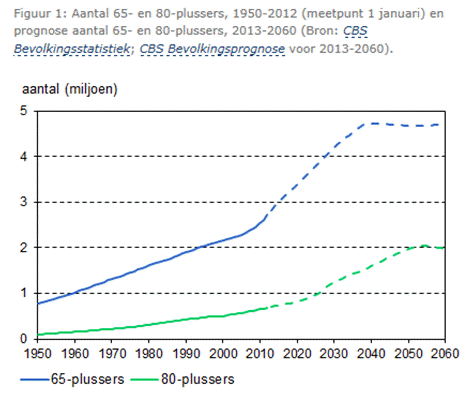
\includegraphics[scale=0.75]{vergrijzing1}
	
	
	
	The amount of elderly people is increasing quickly in the Netherlands. \cite{bevolkingspiramide} The nursing homes can't keep up with the pace and have structural issues. They don't have enough experienced staff and there are a lot of problems with the medication delivery. The elderly also feel that they don't have enough freedom. \cite{structureleproblemen}	 
	
	Because of that, there is a lot of pressure on the caregivers. If we don't reach a solution soon, there will be few places left for new elderly in nursing homes or the quality of care will be lower.
	
	\subsection{Problems With Doors}
	Many of the elderly have difficulities with moving through the nursing home. There are a lot of doors where, for example, elderly in wheelchairs can get stuck because the doors close too quickly. There are also doors which won't open automatically, so they require a caregiver to open it. All these problems take valuable time from the caregiver, who could be doing a lot more important things than opening doors. They also take a lot of time and trouble from the elderly. 
	
	\subsection{Emergency Alert Problems}
	There are also elderly people who have trouble with the emergency alert buttons in the nursing homes. Some of the elderly are paralyzed and have a lot of pain when they're laying in a bad position in bed at night. At those times, they can't reach the emergency alert button and have to wait till morning before they're assisted.
	
	\subsection{Facial recognition and Emotion recognition}
	The way to solve these problems is to use facial recognition for automatically unlocking and opening doors. With facial recognition you could also use emotion recognition to see if elderly people are in pain and need care. 
	
	\newpage
	\section{Solution}
	\subsection{Goals}
	The solution has multiple goals. 
	
	\vspace{5mm}
	The first goal is to make sure the nurses spend less time on opening doors and assisting the elderly through the nursing home.
	
	
	The second goal is to give the elderly more freedom through the building. They don't have to call for a nurse every time for opening doors.
	
	
	The third goal is to detect quickly when an elderly is in pain, so they can be assisted.
	
	\subsection{How It Works}
	All doors have an camera above them connected to a main server. The server runs facial recognition software on all the camera's. The server is also connected to all the doors so they can open automatically.
	
	\newpage
	\section{Concluding}
	
	\newpage
	
	\bibliography{rapport}
	\bibliographystyle{ieeetr}
	


\end{document}